Software testing is a process present in a majority of software developments. According to Mathur's definitions \cite{Mathur2008}, it aims at evaluating if a software behaves as expected. When running a software system, one may face a \emph{\gls{failure}}, \ie an unexpected behaviour of the system. This failure is the propagation to the output of the system of one or more \emph{\glspl{bug}} (also called \emph{\glspl{fault}}), coming from \emph{\glspl{error}} made during the writing of the source code of the software system or resulting from earlier issues in specifications. The goal of a software testing process is to find as many bugs as possible in a given software system, called \acrfull{SUT}, in order to prevent failures to happen during the operation of the software system.

When it comes to product lines, testing becomes more complex. As the system under test is the set of products of this product line, using a standard testing process would require to derive all those products and, for each one of them, design and execute a test suite. This approach, called \emph{product-based} \cite{Thum2014}, is intractable for the large majority of product lines. \gls{SPL} testing requires to adapt standard testing process to minimize the effort by reusing testing assets from one product to another and prioritizing the products to test. To achieve this, most techniques adopt a model-based approach: \eg sampling a set of products to test from a feature model.

This chapter presents the state-of-the-art of SPL testing. Sections \ref{sec:softwaretesting} and \ref{sec:mbt} presents software testing and model-based testing, Section \ref{sec:spltesting} gives a view of \gls{SPL} testing, and Section \ref{sec:mbtspltesting} focuses on existing model-based approach to \gls{SPL} testing.


%%%%%%%%%%%%%%%%%%%%%%%%%%%%%%
\section{Software testing}
%%%%%%%%%%%%%%%%%%%%%%%%%%%%%%

\label{sec:softwaretesting}

The Software Engineering Body of Knowledge from the IEEE Computer Society \cite{swebok2014} defines software testing as follows:
%
\begin{quote}
Software testing consists of the \emph{dynamic} verification that a program provides \emph{expected} behaviours on a \emph{finite} set of test cases, suitably \emph{selected} from the usually infinite execution domain.
\end{quote}
%
This definition, although not specific on how to perform software testing, includes different important aspects. First, the SUT has to be \emph{executed} on a set of input values\footnote{In this case, input values may refer to input data or, more generally, to a specific input state of the SUT.} in order to observe its behaviour. Second, to decide if the SUT behaves as expected, it must be possible, based on the outcomes of the SUT for a given input, to decide if the outcomes are acceptable or not. This is also referred to as \emph{the oracle problem} \cite{swebok2014}. 
Finally, the number of observed behaviours exercised by the test cases is \emph{finite}: a software testing process is the result of a trade-off between limited resources, schedules, and unlimited test requirements. Therefore, the \emph{\gls{test suite}} (\ie the set of test cases) has to be properly selected in order to satisfy this trade-off using a \emph{criterion}.

The software testing process itself may be implemented in various ways. Tretmans~\cite{Tretmans2004,Utting2007} defines a typology of software testing processes based on three dimensions: the characteristic being tested, the scale of the SUT, and the information used to select test cases.

\paragraph{Characteristic being tested:} 
%
The main characteristic being tested is the functionality (\emph{functional testing}), which aims at checking that a SUT produces a correct output for a given input. Other characteristics includes (but are not limited to) robustness (\emph{robustness testing}), which aims at checking that the SUT can resist to invalid conditions in its environment (\eg wrong inputs, hardware failures, network failures, other systems failures, \etc); performance (\emph{performance testing}), which aims at checking that the SUT can resist heavy loads; usability (\emph{usability testing}), which focuses on user interfaces problems; security (\emph{security testing}), which aims at checking that the system is not vulnerable to malicious users; \etc In this thesis, we focus on functional testing.
 
\paragraph{Scale of the SUT:} 
%
It indicates which parts of the system are considered during the execution of each test case: \emph{unit testing} focuses on single units at a time (\eg a single method, a single function, a single class, \etc); \emph{component testing} tests each part of the system separately, while \emph{integration testing} checks that the different components work together correctly; finally, \emph{system testing} considers the whole system to perform testing.

\paragraph{Information used to select test cases:} 
%
Information may be either \emph{white box} or \emph{black box}. White box testing processes use the source code as input. They allow one to define selection criteria on the source code of the application: \eg statement coverage requires that each statement is executed at least once by one test case of the test suite. Black box testing processes will use the requirements of the SUT as input. In this case, the source code is not accessible and selection criteria are specified over the requirements: \eg input domain coverage requires to split the input domain in equivalence classes and to design test cases that will use at least one element of each class.

Most of the time, the selection of a test suite is done manually. For instance, it is very common for developers to write functional unit tests for their code before submitting it to a version control system. In most cases and with the right tool support, this may be enough. However, manual testing becomes expensive for larger systems, especially during integration and system testing \cite{Utting2007}. 

%%%%%%%%%%%%%%%%%%%%%%%%%%%%%%
\section{Model-based testing}
%%%%%%%%%%%%%%%%%%%%%%%%%%%%%%

\label{sec:mbt}

\begin{figure}
	\centering
	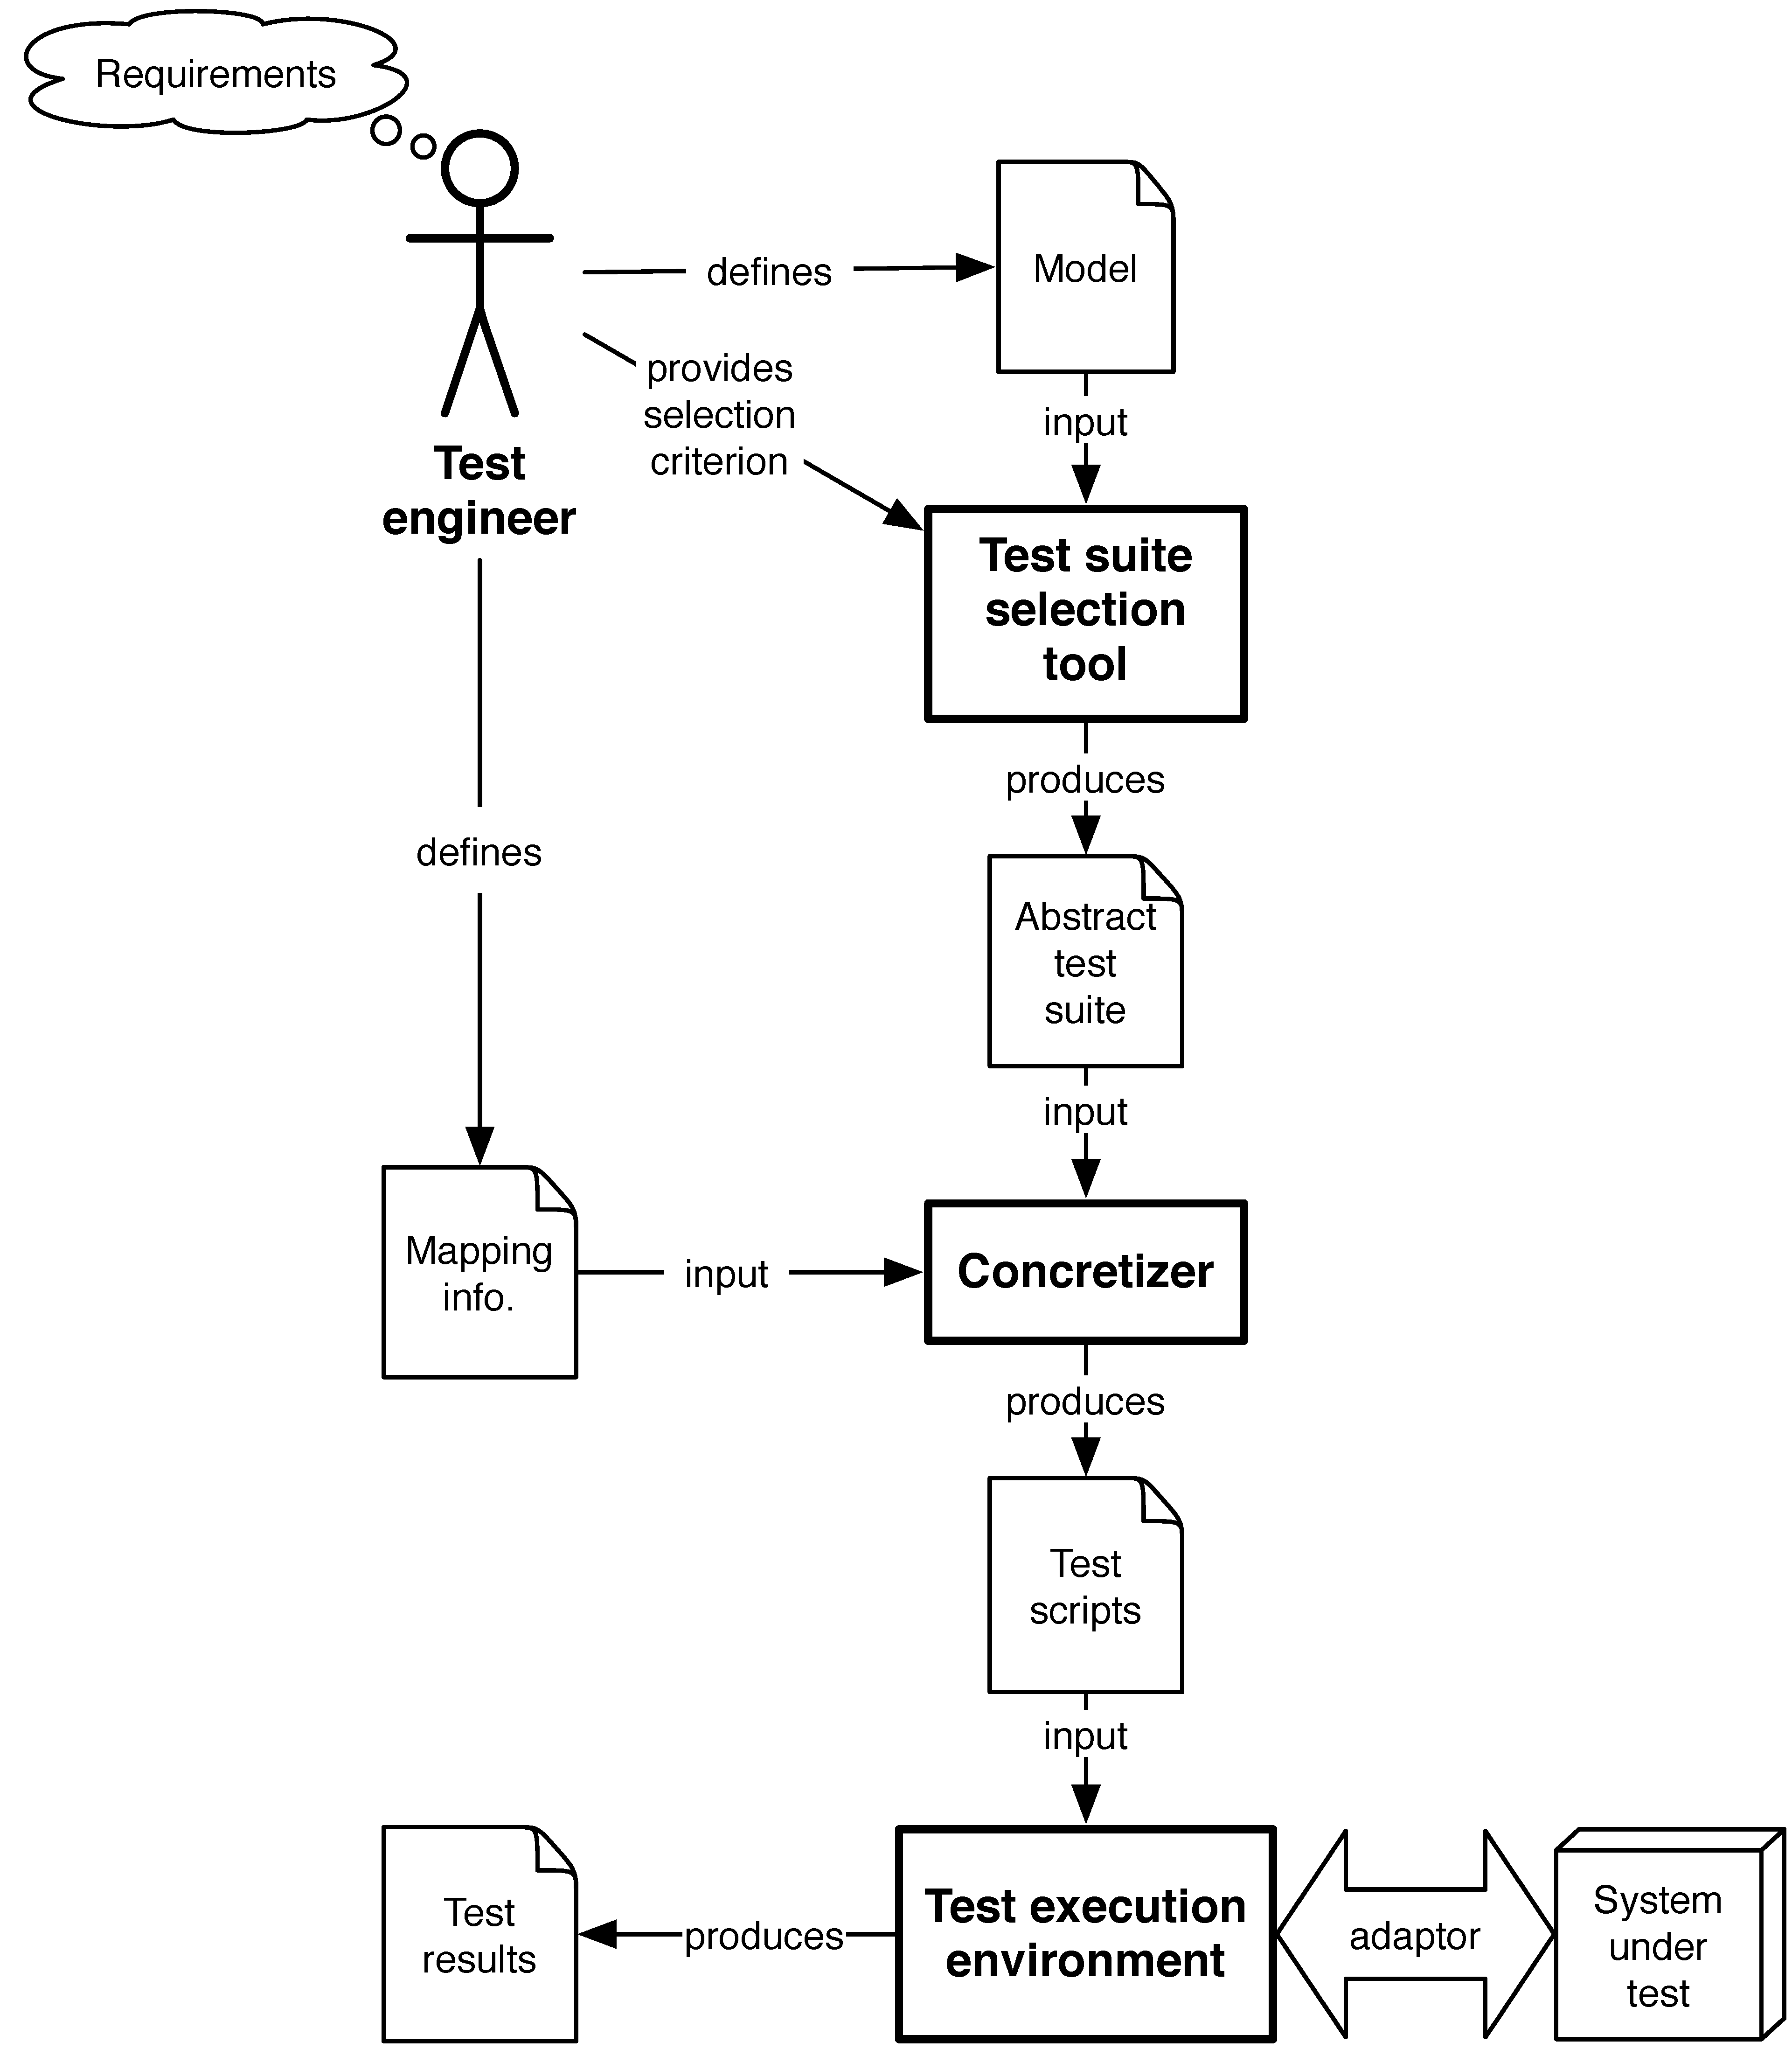
\includegraphics[width=110mm]{mbt-process}
	\caption{Model-based testing process}
	\label{fig:mbtprocess}
\end{figure}

Automating test suite selection is not easy though. It requires an \emph{input generator} that, for each test case, generates a sequence of input operations for the system (\eg a sequence of method calls); an \emph{oracle} which decides, based on the input sequence and the outputs of the system if the test case is pass or fail; and a \emph{selection criterion} (with a mechanism to measure it) in order to decide when to stop the selection. For instance, EvoSuite \cite{Fraser2011} is a white box Java test cases generator that uses an evolutionary algorithm to generate JUnits by analysing methods paths. Since the tool only uses the source code as input, the oracle is very limited and can only tell if a test case execution should throw an exception or not. To improve this oracle, it requires to analyse the specification of the methods to foretell the expected output.

An alternative is to use a semi-automated approach: \emph{model-based testing} \cite{Utting2007}. It requires to define a model of the expected behaviour of the SUT (\ie a specification) that serves as input to an automated test suite selection tool. The model should be small enough to be cheaper than the analysis of the actual system, but accurate enough to describe the characteristics to test. The tool uses this model to generate a sequence of input and as oracle for each sequence. Model-based testing is the automation of black box test suite selection \cite{Utting2007}.

Figure \ref{fig:mbtprocess} presents a generic model-based testing process. First the test engineer defines a \emph{model} of the SUT. This model is provided to the test suite selection tool that, based on the \emph{selection criterion} specified by the test engineer, selects an \emph{abstract test suite}. This abstract test suite contains test cases expressed at the same abstraction level than the input model. They cannot be executed on the SUT as-is and require to be \emph{concretized} to test scripts using mapping information to link abstract actions and inputs in the test cases to concrete SUT operations. The test scripts may then be \emph{executed} by a dedicated test execution environment that operates the SUT (optionally using an adaptor layer to abstract complex SUT's operations) and produces a report with the test results. We present our implementation of this generic process in Chapter \ref{chap:frameworkdescription}.


%%%%%%%%%%%%%%%%%%%%%%%%%%%%%%%%%%%%%%%%
\section{Software product line testing}
%%%%%%%%%%%%%%%%%%%%%%%%%%%%%%%%%%%%%%%%

\label{sec:spltesting}

As presented in Figure \ref{fig:spldev}, \gls{SPL} testing is performed on two different levels: domain testing and application testing \cite{Pohl2005}. During \emph{domain testing}, reusable test artefacts are defined and validated for the SPL. Those artefacts are combined during \emph{application testing} in order to test one particular product. 

%------------------------------------------------------
\subsection{Software product line testing strategies}
%------------------------------------------------------

Domain testing processes include the definition of a test plan corresponding to the strategy used to test the SPL. Pohl \etal \cite{Pohl2005} define four kinds of strategies to validate a \gls{SPL}:

\paragraph{Brute force:} 
%-------------------------------

Brute force strategy consists in performing all the testing activities for all the possible products during domain engineering. 
Considering an \gls{FTS} and a \gls{feature model}, this would consist in deriving all the valid products from the feature model, and for each product, project the FTS on the product to derive test cases from the resulting \gls{LTS} using a classical model-based testing approach \cite{Utting2007}.
As empirically shown by Halin \etal \cite{Halin2017,Halin2017b}, this strategy is expensive, not applicable in most cases, and is no more discussed here.


\paragraph{Pure application:} 
%-------------------------------

Pure application strategy consists in performing testing only during application engineering. Each derived product is tested individually using a standard (non-SPL) testing procedure and no domain test artefacts are reused. Contrary to brute force, pure application strategy does not build all products, it only tests one when it is derived for a customer. 
As for the previous one, an \gls{FTS} may be projected on the considered products and the resulting \gls{LTS} used as input for a model-based testing approach.
This strategy is no more discussed here. Interested reader can refer to single-system software testing literature \cite{Mathur2008,Utting2007}.


\paragraph{Sample application:} 
%-------------------------------

Sample application strategy consists in selecting one or a few sample products (\ie to do a \emph{product prioritization}) to test domain artefacts, but still requires to test other derived products during application engineering. Again, the \gls{FTS} may be projected on the sampled products and the resulting \gls{LTS} used as input for a model-based testing approach. The product sampling itself may be done using various methods: in this thesis, we use the \gls{FTS} to drive it.


\paragraph{Commonality and reuse:} 
%----------------------------------

Commonality and reuse strategy consists in testing parts common to all the products and preparing test artefacts for variable parts during domain engineering, and reusing test artefacts specific to a product during application engineering. Applied to an \gls{FTS} and a \gls{feature model}, this strategy is close to what we propose in this thesis. The mapping information used during abstract test case conretization (in Figure \ref{fig:mbtprocess}) have to be defined for all the actions of the FTS during domain engineering, in order to be reused across different products. To test the parts common to all the products, one has to project the FTS on the product containing only the features common to all the products of the SPL (if it exists) and use the resulting LTS to derive test cases using model-based testing.

On the one hand, \textit{sample application} strategy does not produce variable test artefacts (and thus does not reuse domain test artefacts during application engineering). This may cause an overhead if the sampled products do not correspond to the products derived afterwards. On the other hand, \textit{commonality and reuse} strategy allows to reuse domain test artefacts during application engineering, but validates only parts common to all products during domain testing, lacking at detecting problems in variable parts in an early development stage.
A fifth strategy consists in \emph{combining} \textit{sample application} and \textit{commonality and reuse} strategies: domain test artefacts contains variability information and may be reused and a sample of products is used to test common and variable parts of the product line. This allows to have a faster feedback on variable parts validation while still allowing to reuse domain test artefacts during application testing. This last strategy is the one recommended for the framework developed in this thesis. 

%------------------------------------------------------
\subsection{Software product line analysis classification}
%------------------------------------------------------

To support domain testing, a lot of existing approaches use analysis techniques to select test cases and prioritize products. Depending on the considered artefacts and the modality, Th\"um \etal \cite{Thum2014} classify \gls{SPL} analysis in three categories:

\paragraph{Product-based analysis:} 
%----------------------------------

In product-based analysis, products are built and analysed individually. This allows to use existing methods designed for single systems that will work on application artefacts only, but becomes expensive if the set of products to analyse is large. To overcome this, one may first prioritize products to perform the analysis only on a subset of all the products of the product line. In this case, the product-based analysis is combined with a family-based sampling technique. 

\paragraph{Family-based analysis:} 
%----------------------------------

Family-based analysis uses domain artefacts in combination with a feature model to perform a variability aware analysis of all the products of the product line at once. For instance, FTS model checking \cite{Classen2013b} is a family-based analysis. The ProVeLines \cite{Cordy2013} model checker uses the feature model and the feature expressions on the transitions to check that all the products satisfies the given property in one exploration of the FTS. If this is not the case, it prints the products that violates the property.

\paragraph{Feature-based analysis:} 
%----------------------------------

In feature-based analysis, domain artefacts implementing a given feature are analysed in isolation without considering other features. Contrary to family-based analysis, feature-based does not consider the feature model during the analysis and are not able to detect undesired features interactions \cite{Zave1993} (\ie undesired behaviours appearing only if a certain combination of features is present in the product).

As for SPL testing strategies, analyses may be combined. For instance, performing a feature-based analysis before a product-based or a family-based analysis may reduce the effort needed by the latter as feature-based analysis allows to factorise the analyse of elements that do not depend on other features. In our model-based testing framework, test cases and products are selected from domain artefacts (\ie a \gls{FTS} and a \gls{feature model}) and concretized into executable test scripts in a family-based approach, while the execution of the test scripts on each product is product-based.


%%%%%%%%%%%%%%%%%%%%%%%%%%%%%%%%%%%%%%%%%%%%%%%%%%%%%
\section{Model-based software product line testing}
%%%%%%%%%%%%%%%%%%%%%%%%%%%%%%%%%%%%%%%%%%%%%%%%%%%%%

\label{sec:mbtspltesting}

There exists several testing approaches to software product lines and lot of them are model-based \cite{Oster2011,Engstrom2011,Machado2014}. This may be explained by the complexity induced by the product lines variability. This variability is usually captured in a feature model reused during testing in combination with other domain artefacts (that may be models or not). A large part of those approaches are focused on \emph{sampling} a representative set of products to test in order to find as many undesired feature interactions as possible \cite{Machado2014}. 

%--------------------------------
\subsection{Feature interaction}
%--------------------------------

\glsreset{CIT}

Apel \etal \cite{Apel2013} define a \emph{feature interaction} between at least two features as \textit{an emergent behaviour that cannot be easily deduced from the behaviours associated with the individual features involved}. A lot of those interactions are intended: for instance, a security feature may interact with other features by encrypting all connections. Problem occurs when an \emph{unintended feature interaction} happens, usually resulting from a bug, and causes failures at runtime in the products containing the features involved. Test cases have to check that desired feature interactions are achieved, by checking that connections are encrypted for instance, but also that undesired interactions do not happen.

One of the specificities of software product line testing is thus to seek and find undesired feature interactions, usually occurring when a small number of features are involved \cite{Kuhn2004}. For instance, amongst the 6 faults discovered in JHipster, Halin \etal \cite{Halin2017b} found that 5 are caused by interactions of size two and one by an interaction of size four. To find those undesired feature interactions, sampling techniques have been developed to select a representative set of products involving as many different feature combinations as possible. The most common sampling techniques are based on \emph{\gls{CIT}} and known as \textit{t}-wise product sampling.

%--------------------------------------
\subsection{\textit{T}-wise sampling}
%--------------------------------------

%\begin{table}
%\centering
%\caption{2-wise covering array for the card payment terminal}
%\label{tab:cit:cpterminal}
%\begin{small}
%\begin{tabular}{c | cccccc}
%\textbf{Product} & \textbf{DirectDebit} & \textbf{CreditCard} & \textbf{Online} & \textbf{Offline} & \textbf{Signature} & \textbf{PIN}\\
%\hline
%1 & true 		& true 		& false & false 		& false 		& false \\
%2 & true 		& false 		& true 	& true 		& false 		& false \\
%3 & true 		& true 		& true 	& false 		& true 		& true \\
%4 & false 		& true 		& false	& true 		& true 		& true \\
%5 & false 		& false 		& false	& true 		& true 		& false \\
%6 & false 		& false 		& true 	& false 		& false 		& true \\
%\end{tabular}
%\end{small}
%\end{table}

\textit{T}-wise sampling techniques sample a set of products in which all the \textit{t}-uples of features allowed by the feature model are represented at least once. The parameter \textit{t} is called the \emph{strength} of the sampling. Since lot unintended feature interactions appear between two features \cite{Kuhn2004}, pairwise (2-wise) product sampling is the most studied approach \cite{Lopez-Herrejon2015a,Machado2014}. 

%Initially, \gls{CIT} techniques performing \textit{t}-wise sampling represent this set as a covering array of size $N \times k$, where $k$ is the number of features (\ie the columns of the array) and $N$ is the number of selected products (\ie the lines of the array). Formally, a covering array is defined as follows:
%%
%\begin{definition}[Covering array \cite{Mathur2008}]
%A covering array \textit{CA}$(N, k, s, t)$ is a $N \times k$ array in which entries are from a finite set $S$ containing $s$ symbols such that every $N \times t$ subarray contains all \textit{t}-uples at least once.
%\end{definition}
%
%In a SPL context,  $S = \mathbb{B}$: a feature is \textit{true} if it is selected in a product and \textit{false} otherwise. This definition does not take \emph{constraints} between features into account. For instance, Table \ref{tab:cit:cpterminal} gives the covering array\footnote{The covering array has been generated using CASA \cite{Garvin2009,Garvin2011} without constraints.} of strength 2 for the card payment terminal of Figure \ref{fig:cpterminalsimplifiedfm}. Constraints \textit{Di\-rect\-De\-bit} $\Rightarrow$ \textit{PIN} and \textit{PIN} $\Rightarrow$ \textit{Signature} are violated in the first, second, and last products of Table \ref{tab:cit:cpterminal}.

Many \gls{CIT} approaches have been adapted to take constraints from the feature model into account in order to perform \emph{\textit{t}-wise sampling} \cite{Cohen2008,Lopez-Herrejon2015a}. They are implemented in different tools like CASA \cite{Garvin2009,Garvin2011}, SPLCAT \cite{Johansen2012}, NIST-ACTS \cite{Lei2007}, MoSo-PoLiTe \cite{Oster2010}, PACOGEN \cite{Hervieu2011}, \etc Depending on the approach, a large variety of underlying techniques may be used \cite{Calvagna2013a,Lopez-Herrejon2015a}. 
The main ones \cite{Cohen2008,Lamancha2015} are 
\emph{algebraic methods} \cite{Calvagna2008,Sherwood1994,Hartman2005}, 
\emph{greedy algorithms} \cite{Garvin2009,Garvin2011,Cohen1997,Lott2005a,Czerwonka2006,Sherwood1994,Bryce2009,Bryce2006,Bryce2007,Lamancha2015,Lei2008,Johansen2011,Johansen2012b,Johansen2012}, 
\emph{heuristic search} \cite{Garvin2009a,Cohen2003}, 
and \emph{constraint programming} \cite{Oster2010,Marijan2013,Patel2013,Patel2013a,Hervieu2011,Perrouin2011}.

Despite advances being made, introducing constraints during \textit{t}-wise sampling yields scalability issues for large feature models \cite{Arcuri2012,Grindal2005,Nie2011,Henard2014a} and higher interaction strengths \cite{Kuhn2008,Reisner2010,Petke2013,Henard2014a}. To overcome those limitations, Henard \etal \cite{Henard2014a} developed a dissimilarity-driven sampling to mimic the \textit{t}-wise criteria. This sampling tries to maximise the dissimilarity between the selected products.

%------------------------------------------
\subsection{Dissimilarity-driven sampling}
%------------------------------------------

Dissimilarity-driven product sampling is based on the following heuristic: dissimilar products are more likely to detect bugs than similar ones. This is empirically demonstrated for single systems (model-based) testing by Hemmati \etal \cite{Hemmati2010}. The idea is to sample a set of products as dissimilar as possible, based on a distance measure. In their work, Henard \etal \cite{Henard2014a} consider the \emph{distance} between products in terms of selected features: two products are dissimilar if the features that compose them are different. 

The sampling is performed using an \emph{evolutionary algorithm} that takes a fixed size for the sample and a duration as parameters. The Jaccard distance \cite{Jaccard1901} between two products is used to compute the fitness value of the sample at each iteration. During the execution, products are ranked inside the sample according to their dissimilarity. Eventually, the algorithm produces a ranked list of products where most dissimilar ones are in the first positions. Contrary to \gls{CIT} algorithm, the size of the sample is fixed from the beginning. This may require some prior decision from the test engineer, but is also very convenient when the testing budget is limited to a given number of products \cite{Halin2017b}. 

The algorithm is implemented in PLEDGE\footnote{See \url{http://research.henard.net/SPL/PLEDGE/}.} and Henard \etal \cite{Henard2014a} empirically demonstrate the relevance of dissimilarity-driven sampling for software product lines for large feature models and higher strengths. 
Those results have been independently confirmed for smaller \glspl{SPL} by Al-Hajjaji \etal \cite{Al-Hajjaji2016}. 
Parejo \etal \cite{Parejo2016} extended this idea, using a genetic algorithm, by considering both functional and non-functional properties during the selection process. 
In this thesis, we extend this idea in Chapter \ref{chap:coverage} by considering both features and behavioural dissimilarity during the sampling. More details on distance measure, fitness value, and selection algorithm are provided in this chapter.

%---------------------------
\subsection{Related work}
%---------------------------

Other strategies to  perform SPL mode-based testing at the domain level have been proposed. Lochau \etal \cite{Lochau2012,Lochau2014} define a model-based approach that shifts from one product to another by applying deltas to state-machine models. The approach allows to reuse test cases from previous products and derive of (re)test obligations for each new considered product. These deltas, are built incrementally when switching from one product to another and are part of the reusable domain test artefacts. In this thesis, we want to select relevant test cases and products before performing the effective tests.
%
Cichos \etal \cite{Cichos2011} use the notions of 150\% test model, \ie a test model of the behaviour of a product line, and of test goal to select test cases for a product line but do not define criteria at the SPL level. 
%
Beohar \etal \cite{Beohar2014a} adapt \textit{ioco} \cite{Tretmans2008} to \glspl{FTS}. The Input-Output Conformance (\textit{ioco}) testing is a model-based testing approach that aims at building a conformance relation between a specification and a model of the running system, based on the inputs and outputs of this system \cite{Tretmans2011,Tretmans2008}. Contrary to this approach, we do not seek exhaustive testing of an implementation but rather to select relevant abstract test cases based on the criteria provided by the test engineer.


%%%%%%%%%%%%%%%%%%%%%%
\section{Wrap up}
%%%%%%%%%%%%%%%%%%%%%%

This chapter presents the necessary background on software testing, a generic model-based testing procedure, and the most studied model-based software product line testing approaches. A lot of those approaches are family-based: they use domain artefacts and reason at the product line level. They seek to sample a subset of products to test in priority, based on the feature model and a sampling  criterion. In this chapter, we present \textit{t}-wise and dissimilarity-driven sampling. \textit{T}-wise ensures that every \textit{t} combination of features is present in at least one sampled valid product and dissimilarity-driven try to maximise the dissimilarity (in terms of features) between the sampled products. 

Complementary to those approaches, the selection criteria developed in Chapter \ref{chap:coverage} take not only variability, but also behaviour into account. We define in Chapter \ref{chap:frameworkdescription} a \emph{family-based} model-based testing framework that may be used in \emph{combined \textit{sample application}} and \emph{\textit{commonality and reuse}} testing strategies.

